% -----------------------------------------------
% Template for SMAC SMC 2013
% adapted and corrected from the template for SMC 2012, which was adapted from that of SMC 2011
% further updated for TENOR 2015 and 2016
% -----------------------------------------------

\documentclass{article}
\usepackage{tenor2016}
%\usepackage{times}
\usepackage[utf8]{inputenc}
\usepackage{ifpdf}
\usepackage[english]{babel}
%\usepackage{balance}

%\usepackage{cite}

%%%%%%%%%%%%%%%%%%%%%%%% Some useful packages %%%%%%%%%%%%%%%%%%%%%%%%%%%%%%%
%%%%%%%%%%%%%%%%%%%%%%%% See related documentation %%%%%%%%%%%%%%%%%%%%%%%%%%
%\usepackage{amsmath} % popular packages from Am. Math. Soc. Please use the 
%\usepackage{amssymb} % related math environments (split, subequation, cases,
%\usepackage{amsfonts}% multline, etc.)
%\usepackage{bm}      % Bold Math package, defines the command \bf{}
%\usepackage{paralist}% extended list environments
%%subfig.sty is the modern replacement for subfigure.sty. However, subfig.sty 
%%requires and automatically loads caption.sty which overrides class handling 
%%of captions. To prevent this problem, preload caption.sty with caption=false 
%\usepackage[caption=false]{caption}
%\usepackage[font=footnotesize]{subfig}

\usepackage{verbatim}
\usepackage{color}
\usepackage{textcomp}

\definecolor{mygrey}{gray}{0.93}
\definecolor{figOrange}{RGB}{212,85,0}
\definecolor{figRed}{RGB}{128,0,0}
\definecolor{red}{RGB}{250,0,0}
\definecolor{figBlue}{RGB}{0,136,170}

\newenvironment{ExprCode}		{\vspace{-2mm} \small\verbatim}{\endverbatim\vspace{-2mm}}
\newcommand{\OSC}[1]{\texttt{#1}}
\newcommand{\oper}[1]{\textcolor{figRed}{#1}}
\newcommand{\param}[1]{\textcolor{figOrange}{#1}}
\newcommand{\prefix}[1]{\textcolor{figBlue}{#1}}

\newcommand{\note}[1]{\textcolor{red}{(#1)}}


\newcommand{\sExpr}{\emph{score expressions}}
\newcommand{\SExpr}{\emph{Score expressions}}
\newcommand{\lowTilde}{\texttildelow}
\newcommand{\tab}{\hspace*{4mm}}

\let\olditemize\itemize
\let\oldenditemize\enditemize
\renewenvironment{itemize} 	{\olditemize \setlength{\itemsep}{1mm}}{\oldenditemize}

\newcommand{\sample}	[1]			{\vspace{-0.2em}\begin{center}\colorbox{mygrey}{\begin{minipage}[t]{0.95\columnwidth} {\small \texttt{#1}}\end{minipage}}\end{center}}


%user defined variables
\def\papertitle{INScore expressions to compose symbolic scores}
\def\authors{G. Lepetit-Aimon \qquad D. Fober \qquad Y. Orlarey \qquad S. Letz}
\def\firstauthor{Gabriel Lepetit-Aimon}
\def\secondauthor{Dominique Fober}
\def\thirdauthor{Yann Orlarey}
\def\fourthauthor{Stéphane Letz}

% adds the automatic
% Saves a lot of ouptut space in PDF... after conversion with the distiller
% Delete if you cannot get PS fonts working on your system.

% pdf-tex settings: detect automatically if run by latex or pdflatex
\newif\ifpdf
\ifx\pdfoutput\relax
\else
   \ifcase\pdfoutput
      \pdffalse
   \else
      \pdftrue
\fi

\ifpdf % compiling with pdflatex
  \usepackage[pdftex,
    pdftitle={\papertitle},
    pdfauthor={\firstauthor, \secondauthor, \thirdauthor},
    bookmarksnumbered, % use section numbers with bookmarks
    pdfstartview=XYZ % start with zoom=100% instead of full screen; 
                     % especially useful if working with a big screen :-)
   ]{hyperref}
  %\pdfcompresslevel=9

  \usepackage[pdftex]{graphicx}
  % declare the path(s) where your graphic files are and their extensions so 
  %you won't have to specify these with every instance of \includegraphics
  \graphicspath{{./figures/}}
  \DeclareGraphicsExtensions{.pdf,.jpeg,.png}

  \usepackage[figure,table]{hypcap}

\else % compiling with latex
  \usepackage[dvips,
    bookmarksnumbered, % use section numbers with bookmarks
    pdfstartview=XYZ % start with zoom=100% instead of full screen
  ]{hyperref}  % hyperrefs are active in the pdf file after conversion

  \usepackage[dvips]{epsfig,graphicx}
  % declare the path(s) where your graphic files are and their extensions so 
  %you won't have to specify these with every instance of \includegraphics
  \graphicspath{{./figures/}}
  \DeclareGraphicsExtensions{.eps}

  \usepackage[figure,table]{hypcap}
\fi

%setup the hyperref package - make the links black without a surrounding frame
\hypersetup{
    colorlinks,%
    citecolor=black,%
    filecolor=black,%
    linkcolor=black,%
    urlcolor=black
}


% Title.
% ------
\title{\papertitle}

% Authors
% Please note that submissions are NOT anonymous, therefore 
% authors' names have to be VISIBLE in your manuscript. 
%
% Single address
% To use with only one author or several with the same address
% ---------------
\oneauthor
   {\authors} {Grame \\ %
  Centre nationale de création musicale \\
  Lyon - France \\
     {\tt \href{mailto:gabriel.lepetit.aimon@grame.fr}{gabriel.lepetit.aimon@grame.fr}}}

%Two addresses
%--------------
% \twoauthors
%   {\firstauthor} {Grame \\ %
%     {\tt \href{mailto:gabriel.lepetit.aimon@grame.fr}{gabriel.lepetit.aimon@grame.fr}}}
%   {\secondauthor} {Grame \\ %
%     {\tt \href{mailto:fober@grame.fr}{fober@grame.fr}}}

% Three addresses
% --------------
% \threeauthors
%   {\firstauthor} {Affiliation1 \\ %
%     {\tt \href{mailto:author1@adomain.org}{author1@adomain.org}}}
%   {\secondauthor} {Affiliation2 \\ %
%     {\tt \href{mailto:author2@adomain.org}{author2@adomain.org}}}
%   {\thirdauthor} { Affiliation3 \\ %
%     {\tt \href{mailto:author3@adomain.org}{author3@adomain.org}}}


% ***************************************** the document starts here ***************
\begin{document}

\capstartfalse
\maketitle
\capstarttrue
%
\begin{abstract}
INScore is an environment for the design of augmented interactive music scores turned to non-conventional use of music notation. The environment allows arbitrary graphic resources to be used and composed for the music representation. It supports symbolic music notation, described using Guido Music Notation or MusicXML formats. The environment has been extended to provided score level composition using a set of operators that consistently take scores as arguments to compute new scores as output. INScore API supports now \sExpr\ both at OSC and at scripting levels. The work is based on a previous research that solved the issues of the notation consistency across scores composition. This paper focuses on the language level and explains the different strategies to evaluate score expressions.
\end{abstract}
%

\section{Introduction}\label{sec:introduction}

Contemporary music creation poses numerous challenges to the music notation. Spatialized music, new instruments, gesture based interactions, real-time and interactive scores, are among the new domains that are now commonly explored by artists. 
Classical music notation doesn't cover the needs of these new musical forms and numerous research and approaches have recently emerged, testifying to the maturity of the music notation domain, in the light of computer tools for music notation and representation.
Issues like writing spatialized music \cite{Ellberger_tenor2015}, addressing new instruments \cite{tmays:2014} or new interfaces \cite{kschlei:2015} (to cite just a few), are now subject of active research and proposals.

Interactive music and real-time scores are also representative of an expanding domain in the music creation field. The advent of the digital score and the maturation of the computer tools for music notation and representation constitute the basement for the development of this musical form, which is often grounded on non-traditional music representation \cite{RSmith_tenor2015} \cite{Hope_tenor2015} but may also use the common music notation \cite{Hoadley12,hoadley14}. 

In order to address the notations challenges mentionned above, INScore \cite{Fober:12a,fober14c} has been designed as an environment opened to non-conventional music representation (although it supports symbolic notation), and turned to real-time and interactive use \cite{Fober:13b, Fober:14b}. It is clearly focused on music representation only and in this way, differs from tools integrated into programming environments like Bach \cite{agostini12b} or MaxScore \cite{didko08}. 

INScore has been extended with \sExpr\ that provide symbolic scores composition features (e.g., putting scores in sequence or in parallel). Building new scores from existing scores at symbolic  level is not new. Haskell is providing such features \cite{Quick:2013:GAM:2505341.2505345}. Freeman and Lee proposed score composition operations in a real-time and interactive notation context \cite{Lee:2013}. Regarding the score operations used by INScore, they are imported from a previous work \cite{fober12b} that was focusing on the music notation consistency through arbitrary composition. 

The novelty of the proposed approach relies on the dynamic aspects of the scores composition operations, as well as on the persistence of the score expressions. A score may be composed as an arbitrary graph of score expressions and equipped with a fine control over the changes propagation.

The paper introduces first the score composition expressions. Next, the different evaluations strategies are explained and illustrated with examples. The articulation with the INScore environment is presented in detail and followed by concrete use cases. A generalization of this approach is finally proposed in the concluding section.  


\section{Language Specification}\label{language}
\label{languageSpec}
The main idea behind the project is designing a relevant language that provides easy to use tools to compose and to manipulate scores. Indeed, as all the operators have already been defined by the GuidoAR library \cite{fober12b}, the point is to imagine a handy way to use them from INScore's scripts.

\subsection{The operators}

\begin{table*}[htdp]
\begin{center}
\begin{tabular}{rll}
\hline
operation & arguments		&	description \\
\hline
seq 	&	$s1\ s2$		& puts the scores $s1$ and $s2$ in sequence \\
par 	&	$s1\ s2$		& puts the scores $s1$ and $s2$ in parallel \\ 
rpar	&	$s1\ s2$		& puts the scores $s1$ and $s2$ in parallel, right aligned \\
top 	&	$s1\ s2$ 	& takes as many voices as $s2$ contains from $s1$, starting by the top voice \\
bottom 	&	$s1\ s2$ 	& takes as many voices as $s2$ contains from $s1$, starting by the bottom voice  \\
head	& 	$s1\ s2$	& takes the head of $s1$ up to $s2$ duration \\
evhead 	&	$s1\ s2$	& id. but on events basis i.e. the cut point is specified by $s2$ events count \\
tail	&	$s1\ s2$ 	& takes the tail of a $s1$ after the duration of $s2$ \\
evtail 	&	$s1\ s2$ 	& id. but on events basis i.e. the cut point is specified by $s2$ events count \\
transpose 	&	$s1\ s2$	& transposes $s1$ so its first note of its first voice match $s2$ one \\
duration 	&	$s1\ s2$	& stretches $s1$ to the duration of $s2$  \\
			& 	& if not used carefully, this operator can output impossible to display rhythm\\
pitch 	&	$s1\ s2$	& applies the pitches of $s1$ to $s2$ in a loop \\
rhythm 	&	$s1\ s2$	& applies the rhythm of $s1$ to $s2$ in a loop \\
\hline
\end{tabular}
\end{center}

\caption{INScore operators}
\label{operations}
\end{table*}

All the operators have a common interface: regardless their actual definition, they always take two scores as input to produce a score as output. The scores are expressed using the Guido Music Notation format [GMN]\cite{hoos98}. A few low-level score manipulation operations are defined (which apply perfectly to INScore language's philosophy) with a deterministic behaviour (none of the operators implement random operations). However, the limited number of operators can't be a limitation, as the uniformity between their inputs and output make them easy to combine into pipelines designs, creating more high-level operators.

See Table~\ref{operations} for a definition of all the operators.

\subsection{Designing a creative language}
In the context of software used for artistic creation like INScore, designing a language is not trivial. Like any other creative tools,  the \sExpr\ language shall inevitably frame the creation process through which the artist must go. To that extent, conceiving a language is actually designing a creative "work-flow" that the users shall then adopt.

The continuity between inputs and outputs through guido operators allows to compose a music by successively transform and aggregate scores fragments. This process (applying transformations on various materials and combining them into a whole creation) is similar to electro-acoustic creative processes where, after choosing samples, the composer applies effects, equalizer... and mixes them together until the raw musical materials become unrecognisable \note{il faudrait une référence}.

Adapting this approach to the traditional music notation would not only make the language easy to learn for composer (used to the audio pipelines design) but could offer great tools for composition: carving and assembling score samples using structural operators, placing the musical structure
%architecture
 in the center of the creative process. In some ways, the art wouldn't emerge from the quality of the raw score fragments but from the process that transforms, shapes, and links them together. Unlike traditional music composition, the structure couldn't only be a classic expected frame any more, but could be the place where the aesthetic lies.

It's with this perspective of audio pipelines and emphasis of the structure that the \sExpr\ syntax has been defined. In particular, these expressions should make use of various heterogeneous materials including \sExpr\ or existing score objects.

\subsection{\SExpr\ syntax}
\smallbreak
\SExpr\ can be defined using two syntaxes:
\begin{center}
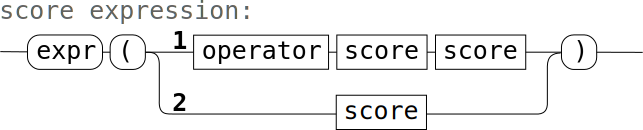
\includegraphics[width=0.9\columnwidth]{imgs/syntax1}
\end{center}

\begin{enumerate}
\item The classic syntax reflects the way Guido operators actually work: two scores are combined into one, according to the operator.
\item The alternate syntax defines an expression using a single score, which can be useful to duplicates objects.
\end{enumerate}

\smallbreak

Both of the syntaxes make use of \OSC{score} arguments. \SExpr\ are quite permissive regarding to their types:
\begin{center}
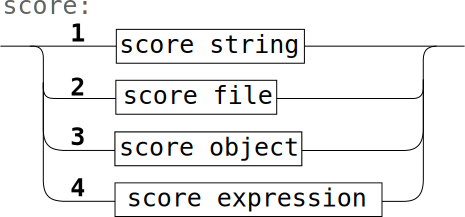
\includegraphics[width=0.7\columnwidth]{imgs/syntax2}
\end{center}

\begin{enumerate}
\item \OSC{score string}: \emph{Guido} or \emph{MusicXML} string.
\item \OSC{score file}:  the content of a \emph{Guido} or \emph{MusicXML} file can be imported using absolute or relative path.
\item \OSC{score object}:  refers to an existing \emph{score object} using a relative or absolute OSC address. \emph{Score object} should be a guido, musicxml or piano-roll object, as well as guido and piano-roll stream object.
\item \OSC{score expression}:  \SExpr\ can be used as arguments inside \sExpr\ (in this case the \OSC{expr} token is optional).
\end{enumerate}

Here is an example of a \emph{score expression} that puts a score in parallel with 2 scores in sequence:
\sample{expr( par score.gmn (seq "[c]" score) )}


%--------------------------------------------
\section{Evaluation Specification}
\label{evaluationSpec}
The \sExpr\ language is first transformed into an internal memory representation. In a second step, this representation is evaluated to produce Guido Music Notation [GMN] \cite{hoos98} strings as output, that are finally passed to the INScore object as specific data.

\subsection{Internal representation of \sExpr}

When encountering an \sExpr, the INScore parser creates a tree representation of it: arguments are stored as leaves and operators as nodes (Figure \ref{fig:parsing}). This tree form allows to easily  store, manipulate, assemble and evaluate \sExpr.

\begin{figure}[th]
\centering
\OSC{ expr( \oper{par} \param{score.gmn}  (\oper{seq} \param{"[c]" score})}
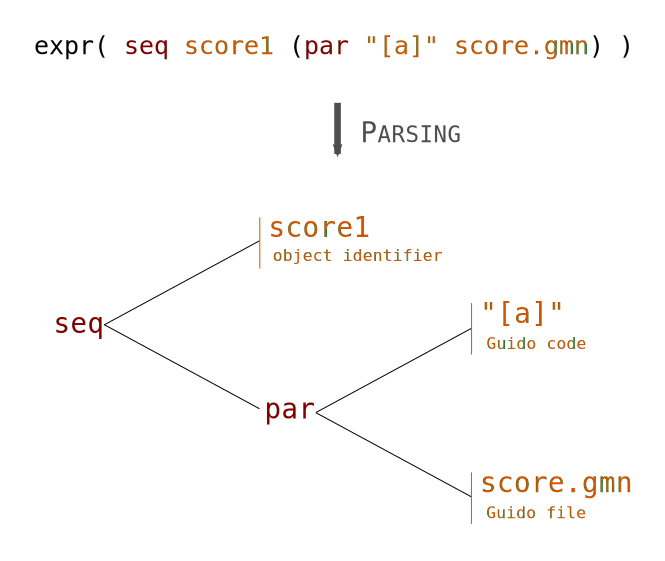
\includegraphics[width=0.8\columnwidth]{imgs/exprParse}
\caption{Parsing \sExpr\ into tree form.
\label{fig:parsing}}
\end{figure}

The tree representation is strictly matching the expression string. Type specification of arguments is the only difference, whereas types are implicit in \sExpr, arguments are explicitly stored as Guido code or file or identifier... in the tree form. 

Once the internal representation has been constructed by the parser, it is stored with the newly-defined object, ready for evaluation.

\subsection{\SExpr\ evaluation process}
During the evaluation process, the evaluator goes through every nodes of the expression tree using a depth first post-order traversal, reducing all of them into GMN code.
A node evaluation is type dependent (Figure \ref{fig:classicEval}). \\
Evaluation of:  
\begin{itemize}
\item a GMN file gives its content,
\item a GMN string returns the string,
\item a MusicXML file returns its content converted to GMN code,
\item a MusicXML string returns the string converted to GMN code,
\item an object identifier gives its GMN code,
\item an operator node returns the application of the operator to the GMN code given as parameters.
\end{itemize}

\begin{figure}[th]
\centering
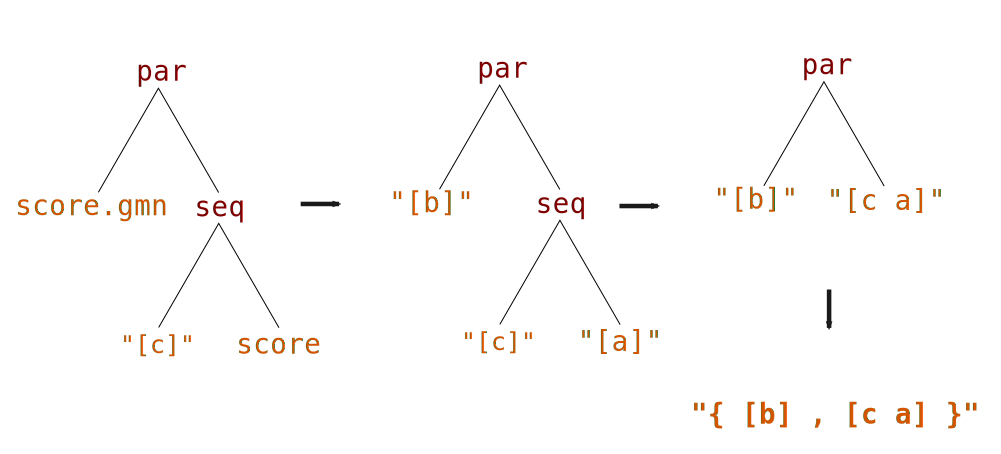
\includegraphics[width=1\columnwidth]{imgs/classicEval}
\caption{Simple evaluation of an expression tree,
where \OSC{score} is defined as \OSC{[a]}
and \OSC{score.gmn} contains \OSC{[b]}.
\label{fig:classicEval} }
\end{figure}

This evaluation scheme avoid recursion issues (e.g. a score that modifies itself using an expression based on its content) since the caller object is modified only at the end of the evaluation process. All arguments are referential transparent by default: each argument is evaluated once and its value is then considered constant.

\subsection{Dynamic evaluation of \sExpr}
%For optimisation and usability reasons, every object defined using a \emph{score expression} store a copy of its tree, so the user can retrieve it later or ask for a re-evaluation when ever he wants. 

Referential transparency (i.e. static evaluation) can be a huge limitation. For example, working with guido stream, one could want to maintain the result of a \emph{score expression} up to date to the stream's actual state and not keep its initial value (most of the times an empty GMN string).
Thus, part of an expression tree can be specified to be evaluated dynamically by prefixing the variable arguments with an \OSC{\&}. When a re-evaluation is triggered (see \ref{exprMsgs}), INScore should check if they have changed, and recompute the expression if so. Only arguments subject to changes (\OSC{score object} or \OSC{score file})  can be declared dynamic.

To optimize the process, all values (arguments and operators) computed during the evaluation process are cached, this way static branches don't have to be evaluated again and dynamic branches are computed again only if needed (if the cached value of a dynamic argument doesn't match the current one). To be sure that only branches that are likely to change are re-evaluated, the operators nodes are also marked as \emph{dynamically} or \emph{statically} evaluated, according to their arguments. They are considered \emph{static} by default 
%(they should never be re-evaluated)
, unless at least one of their arguments is \emph{dynamically evaluated}, in which case they are considered \emph{dynamic}.

\begin{figure}[th]
\centering
\OSC{ expr( \oper{par} (\oper{seq} \param{score.gmn} \prefix{\&}\param{score}) \\
 \tab\tab\tab\tab (\oper{seq} \param{"[a]" score}) )}
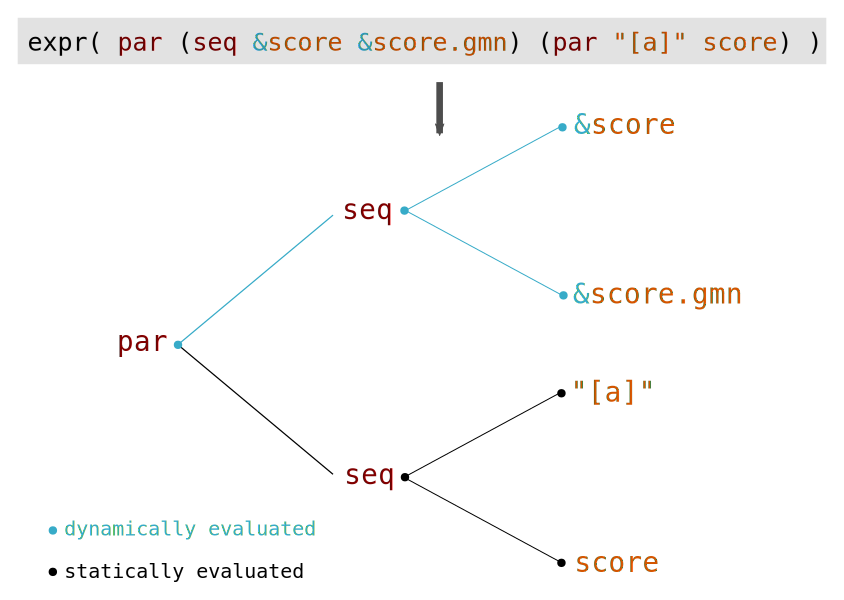
\includegraphics[width=0.9\columnwidth]{imgs/dynamicEval}
\caption{Propagation of dynamic evaluation. \OSC{\prefix{\&}\param{score}} should be updated to the actual value of \OSC{score} when re-evaluating, while \OSC{\param{score}} should keep the value computed on the first evaluation. Thus, on re-evaluation the second \OSC{\oper{seq}} should not be computed again. 
\label{fig:dynamicEval}}
\end{figure}



%--------------------------------------------
\section{Score expressions API in INScore}
\label{exprAPI}
In order to fully integrate score operators, the implementation relies on INScore existing features. As a result, \sExpr\ support URLs as file arguments, interaction events and benefit of web features. Interaction events have been extended notably for the purpose of dynamic evaluation (see section \ref{exprEvents}).

\subsection{Declaring \sExpr}
\label{declaringExpr}
Both \OSC{gmn} and \OSC{pianoroll} objects can be defined with \sExpr\ using an extension of the \OSC{set} message. The evaluation of the expression is actually triggered by the target object when the \OSC{set} message is processed.

\sample{/ITL/scene/score set gmn expr(score.gmn);
/ITL/scene/pr set pianoroll expr(\&score);
}

The previous example creates two objects: \OSC{score} is a symbolic representation of the GMN file \OSC{score.gmn}, and \OSC{pr} is a piano roll representation of \OSC{score} (here dynamically evaluated due to the \OSC{\&} prefix).


\subsection{\SExpr\ specific messages}
\label{exprMsgs}
Objects that that are based on \sExpr\ support additional messages:

\begin{itemize}
\item \OSC{reeval}: triggers the re-evaluation of the expression tree (check if any of the dynamically evaluated arguments should be updated).
\item \OSC{renew}: triggers the re-evaluation of the expression tree regardless of existing constant values. 
\end{itemize}

All these messages are available through the \OSC{expr} message:
\sample{/ITL/scene/score expr reeval;
/ITL/scene/score expr renew;
}

Finally, an object \emph{score expression} can be retrieved with the \OSC{get expr} message:
\sample{/ITL/scene/score get expr;}

\subsection{Events typology extension}
\label{exprEvents}

INScore interaction features are based on the association between an event and arbitrary set of OSC messages \cite{Fober:13b}. These messages are triggered when the event occurs (e.g. a mouse down).
The events typology has been extended with a new event: \OSC{newData}, which is triggered when the value of the target object changes (either due to a \OSC{set} or \OSC{reeval} message, or because data has been written in a stream object).

Associating the \OSC{expr reeval} message to the \OSC{newData} event, produces the automatic reevaluation of an expression when the target object changes:
\sample{/ITL/scene/score set gmn "[a]";\\
/ITL/scene/copy set gmn expr(\&score);\\
/ITL/scene/score watch newData\\   
\hspace*{8mm}(/ITL/scene/copy expr reeval);
}
In the previous example, changing the value of \OSC{score} will automatically change the value of \OSC{copy}.

To catch with infinite loop issues, \OSC{newData} event handling is postponed to the next INScore time slot. As a result, updating the whole scene after changing the value of an object can take several event loop (if one object is referring to another object, itself referring to another one...) and during this process the INScore's graphic scene could go through transitory states. However, if objects are defined with recursive references and are auto-updated using this mechanism, INScore will still be able to update the score (without freezing).

\section{Composing Score Expressions}
\label{composingExpr}
 While the tools already presented allow to compose symbolic scores, it is also possible to compose \sExpr\ which are stored in the referred objects using the prefix \OSC{\prefix{\lowTilde}}. Indeed, whereas \OSC{\param{score}} and \OSC{\prefix{\&}\param{score}} refer to the object's value, \OSC{\prefix{\lowTilde}\param{score}} refers to the \emph{score expression} used to define \OSC{score}. In practical, before the first evaluation, all arguments prefixed by \OSC{\prefix{\lowTilde}} are replaced by a copy of the expression tree from the corresponding objects (Figure \ref{fig:expandingTree}).
It allows to easily make use of previously defined \sExpr\ to create more complex ones.

\begin{figure}[th]

\sample{/ITL/scene/score set gmn\\
\tab expr(\oper{seq} \param{"[a]"} \prefix{\&}\param{sample});\\
/ITL/scene/score set gmn  \\
\tab expr(\oper{seq} (\oper{seq} \prefix{\lowTilde}\param{score} \param{"[b]"}) \prefix{\lowTilde}\param{score});
}

\centering
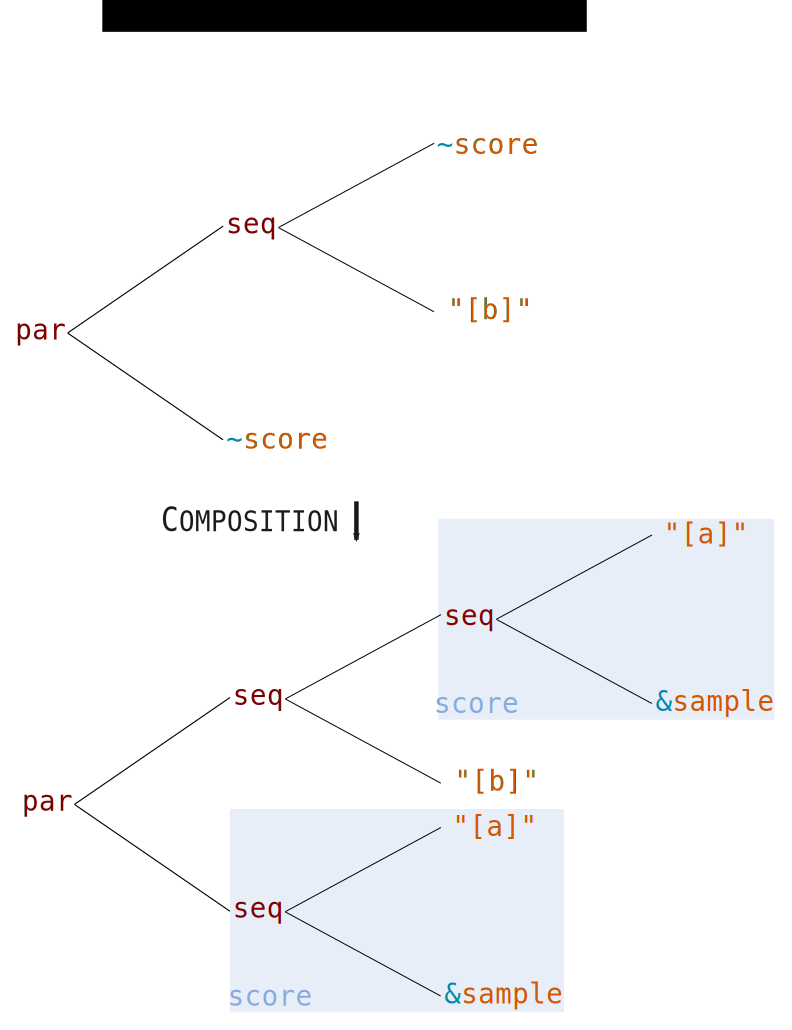
\includegraphics[width=0.9\columnwidth]{imgs/expandingTree}
\caption{Expanding \sExpr\ trees
\label{fig:expandingTree}}
\end{figure}


%------------------------------------------
\section{Examples}
\label{examples}

\subsection{Canon structure}

A simple but still well-known music structure is of course the canon. Creating such structure from a \OSC{score} is quite easy using the \sExpr\ formalism.

\sample{/ITL/scene/score set gmn score.gmn;\\
\\
\# Transposing score\\
/ITL/scene/canon set gmn\\
\tab expr(evtail\\
\tab\tab(transpose\\
\tab\tab\tab(seq "[c]" \&score)\\
\tab\tab\tab"[g]")\\
\tab\tab"[a]"\\
\tab);\\
\\
\# Putting score in sequence with it
/ITL/scene/canon set gmn\\
\tab expr(seq \&score \lowTilde canon);\\
\\
\# Adding a second voice delayed\\
/ITL/scene/canon set gmn\\
\tab expr(par\\
\tab\tab \lowTilde canon\\
\tab\tab (seq "[\_/2]" \lowTilde canon)\\
\tab);
}
The first line import a score into \OSC{score}. Then we transpose it to a fifth and adding a second voice delayed of half a measure. Because transposing according to a specific interval is not a basic guido operator, one should combine \OSC{transpose} with \OSC{seq} and \OSC{evtail} to prepend the score with a note, transpose the whole score using this note and finally remove it.

The result is a simple canon:
\begin{figure}[th]
\centering
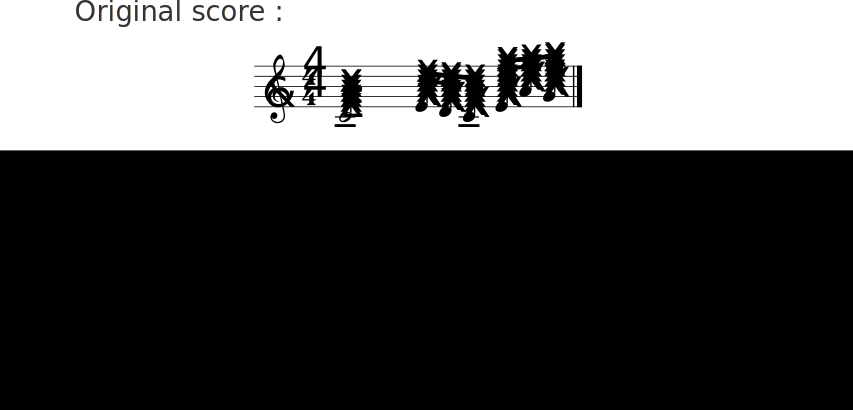
\includegraphics[width=1\columnwidth]{imgs/exampleCanon}
\caption{Canon result
\label{fig:canonFig}}
\end{figure}

\subsection{Multiform but still synced scores}
\SExpr\ is a great tools to duplicate and dynamically transform scores, keeping every copies synced to the original.

\sample{/ITL/scene/origin set gmnf score.gmn;\\
/ITL/saxo/score set gmn \\
\tab expr( evtail\\
\tab \tab (transpose\\
\tab \tab \tab (seq\\
\tab \tab \tab \tab "[e\&1]"\\
\tab \tab \tab \tab \&/ITL/scene/origin )\\
\tab \tab \tab "[c2]" )\\
\tab \tab "[a]"\\
\tab );\\
\\
/ITL/audience/score set pianoroll \\
\tab expr( \&/ITL/scene/origin);\\
\\
/ITL/scene/origin watch newData\\
\tab(/ITL/*/score expr reeval);
}

The previous example create 2 copies of the same score \OSC{origin}, one transposed for saxophones and the other show a piano roll version of \OSC{origin} used as a visual support for the audience.
The last line ensure the update of the copies when \OSC{origin} is modified.

\begin{figure}[th]
\centering
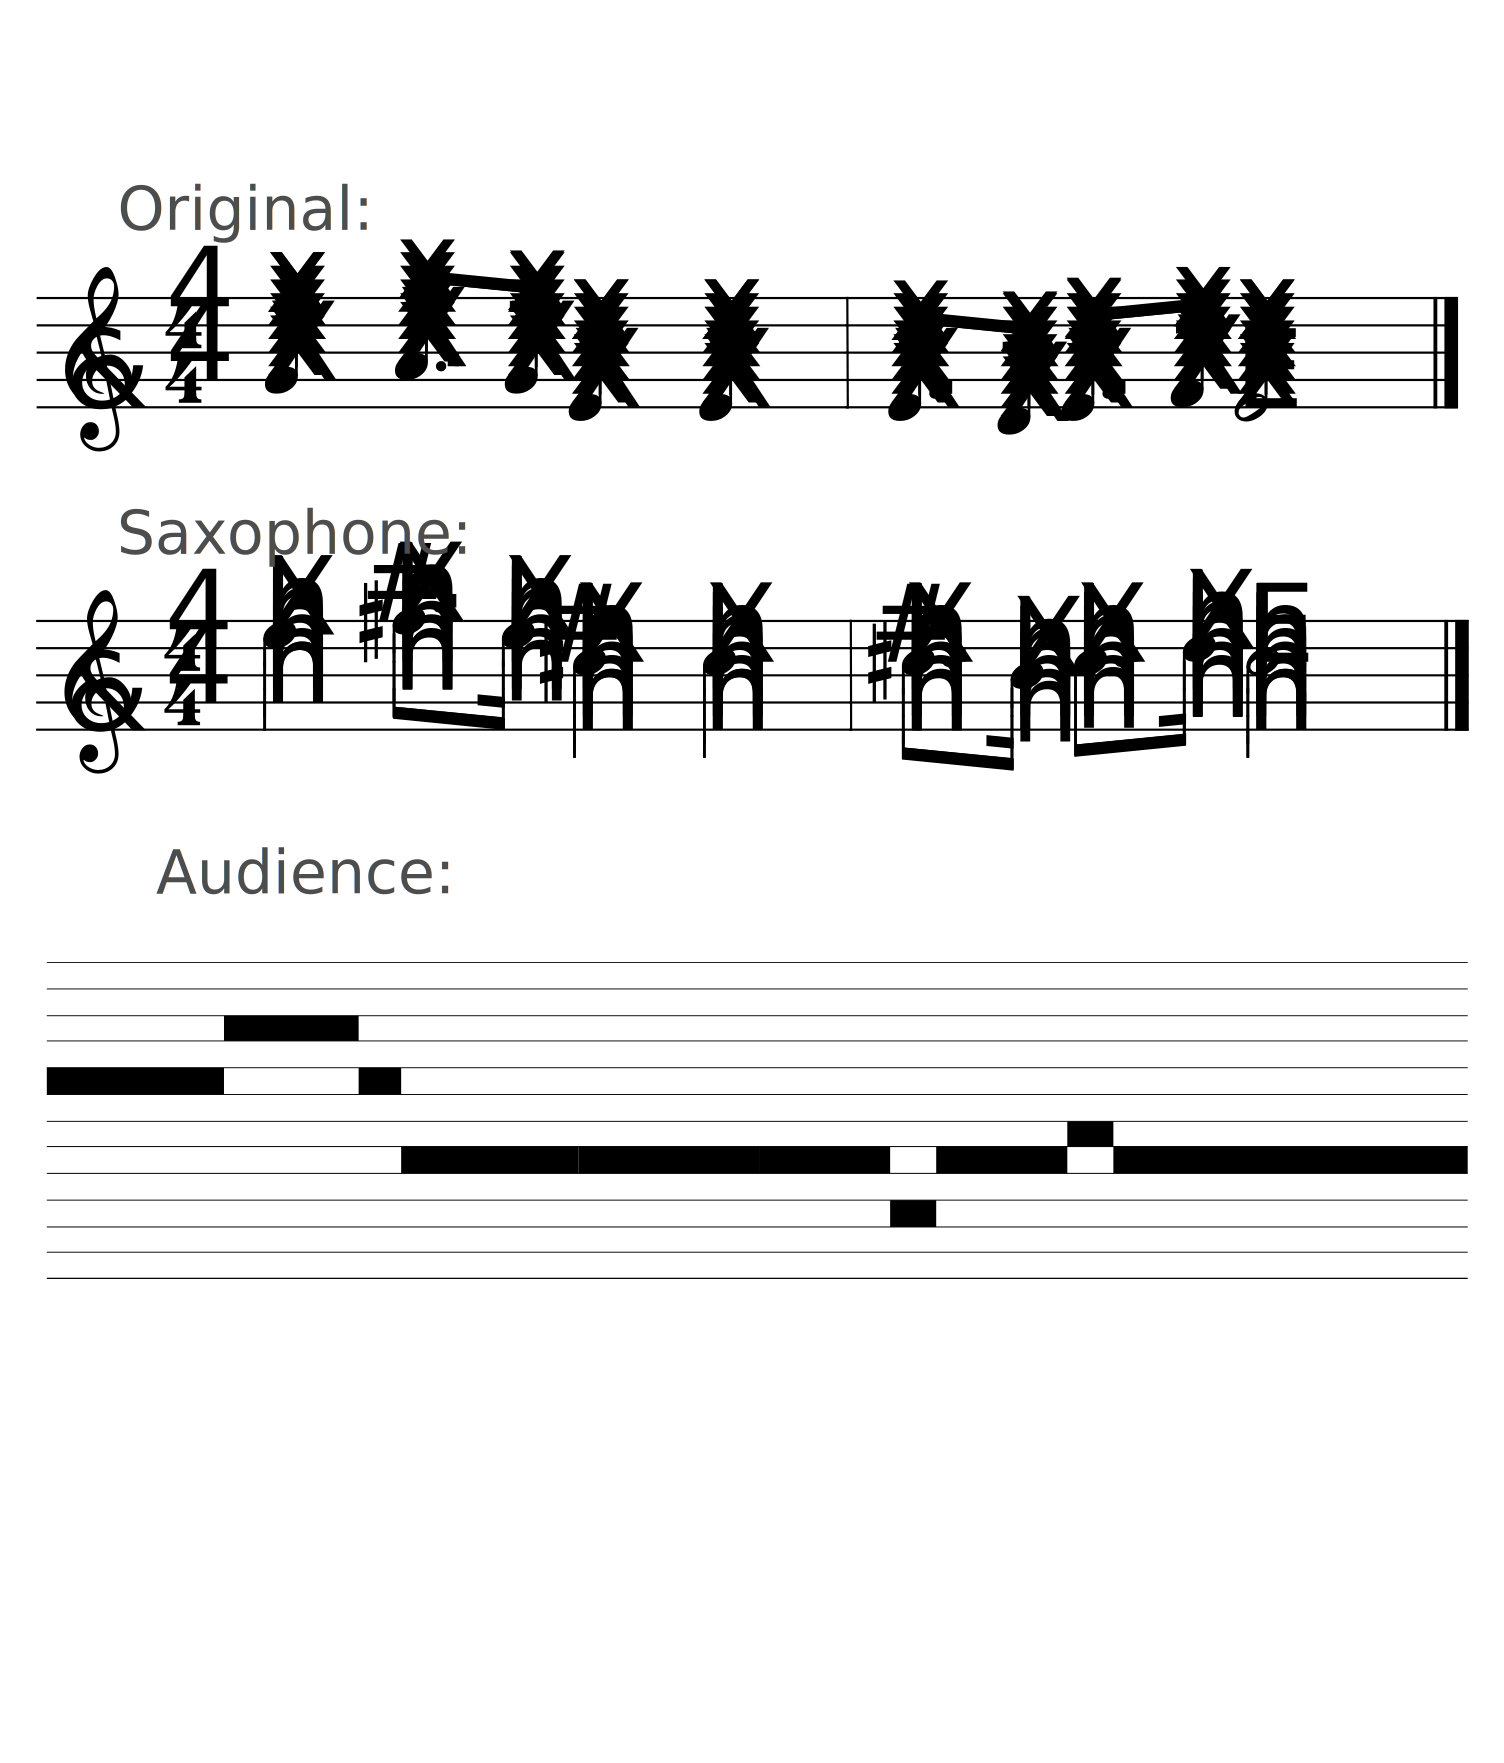
\includegraphics[width=0.8\columnwidth]{imgs/example1}
\caption{Multiform scores result
\label{fig:mutliscoreFig}}
\end{figure}

\section{Conclusions}

Combining the simplicity of GuidoAR operators with the powerful features of INScore (like URL support, full OSC compatibility, interaction support...), \sExpr\ fully integrate score composition into the interactive and augmented music score software. They suggest a creative process based upon musical structures and scores aggregation by giving the possibility to compose various score materials including score objects and even themselves. Above all, \sExpr\ provides a handy tool to manipulate scores regardless to their origins (files, URL, streams...) or their representations (traditional music notation or piano roll).

Still, the implementation process is not over yet, venturing to the traditional music representation's frontiers. Because traditional notation and piano roll representation is not the only ways to write music, because non-conventional music notation make use of a wider variety of shapes or graphics, the \sExpr\ logic should be extended to manipulate any graphical objects of INScore.


\begin{acknowledgments}
You may acknowledge people, projects, 
funding agencies, etc. 
which can be included after the second-level heading
``Acknowledgments'' (with no numbering).
\end{acknowledgments} 

%%%%%%%%%%%%%%%%%%%%%%%%%%%%%%%%%%%%%%%%%%%%%%%%%%%%%%%%%%%%%%%%%%%%%%%%%%%%%
%bibliography here
%\balance
\bibliography{../interlude}

%\begin{ExprCode}
%scoreExpression: 
%		"expr(" operator score score ")"
%      | "expr(" simpleScore ")"
%only inside a score expression context:
%      | "(" operator score score ")"  
%      ;
%               
%score : scoreExpression
%      | simpleScore
%      ;
%      
%simpleScore: GuidoString
%           | MusicXmlString
%           | filepath
%           | "&" filepath
%           | objectIdentifier
%           | "&" objectIdentifier
%           | "~" objectIdentifier
%           ;
%\end{ExprCode}

\end{document}

